\input preamble.tex
\noindent
\section*{Læringsoppdrag Ultralydtransmitter}

\vskip 5pt
%beskrivelse av oppgaven
I dette læringsoppdraget skal du bygge en ultralyd transmitter. Først skal du koble opp og lære om hvordan de ulike delene av transmitteren virker så skal selv sette isammen delene til en transmitter. Du kan til en vis grad velge nivå, ved å velge hvor mange funksjoner du legger inn i den ferdige transmitteren. 

Før du  starter med å sette sammen til en transmitter skal du utføre følgende oppkoblinger mot arduino Nano:
\begin{itemize}[noitemsep]
	\item HC-SR04 ultralyd distanse sensor. 
	\item Oled display
	\item ADC MCP4725
	\item pushbutton rotary encoder
\end{itemize}


\vskip 2.5pt 
Noen av 
%kompetansemål som oppgaven dekker
Kompetansemål:
\begin{itemize}[noitemsep]

	\item planlegge, utføre, vurdere kvalitet, sluttkontrollere og dokumentere arbeidet
	\item planlegge, programmere, montere og idriftsette programmerbare styresystemer
	\item endre og tilpasse skjermbilder for grensesnitt mellom menneske og maskin
	\item anvende ulike elektroniske kommunikasjonssystemer i automatiserte anlegg
	\item vurdere datasikkerhet i automatiserte anlegg
	\item montere, konfigurere, kalibrere og idriftsettelse digitale og analoge målesystemer
	\item måle fysiske størrelser i automatiserte anlegg
	\item feilsøke og rette feil i automatiserte anlegg
	\item dokumentere egen opplæring i automatiseringssystemer
\end{itemize}

%anbefalt lesning til arbeidsoppdragene
Anbefalt lesning:

\begin{enumerate}
	\item afgv.pdf/ 
\end{enumerate}

%Liste over oppdrag som skal gjøres med ruter for godkjennening

%\begin{center}
%\begin{tabular}{ | m{10cm} | m{1cm}| m{2cm} | } 
%\hline
%\multicolumn{3}{|c|}{Liste over oppgaver som skal utføres} \\
%	\hline
%	Oppgave	& Utført & Signatur \\ 
%	\hline
%	\hline
%	(Nivå 1)	& & \\ 
%	\hline
%	(Nivå 2)	& & \\ 
%	\hline
%	(Nivå 3)	& & \\ 
%	\hline
%	(Nivå 4)	& & \\ 
%	\hline
%\end{tabular}
%\end{center}

%--------------------------------------
\newpage

\subsection*{Oppgave 1 -  Oppkobling av HC-SR04}
I denne oppgaven skal vi bli kjent med ultralydsensoren HC-SR04. Denne sensoren sender ut en ultralyd puls når Trig pinnen akriveres (10µs puls), sammtidig som trig pinnen aktiveres slås echo pinnen på. Denne står på til vi mottar et retur signal (reflektert lyd)

$$\includegraphics[width=9cm]{./lUltralydtransmitterx03.eps}$$
I vårt program kan vi bruke funksjonen \verb|pulseIn()|. Denne funksjonen tar tiden på hvor lenge en variabel (echo pinnen) har vært høy. Den virker på pulser fra 10µs til 3 minutter. Tiden den returnerer er i µs. 
\vskip 2.5pt 

Du kan starte med å koble sammen Arduino Nano og HC-SR04 ultralyd sensor slik:
$$\includegraphics[width=8cm]{./lUltralydtransmitterx04.eps}$$
Skriv inn denne koden i Arduino IDE og legg den inn på en Arduino Nano. Det er mulig du må bruke old bootloader. Prøv dette om opplasting ikke virker. 
$$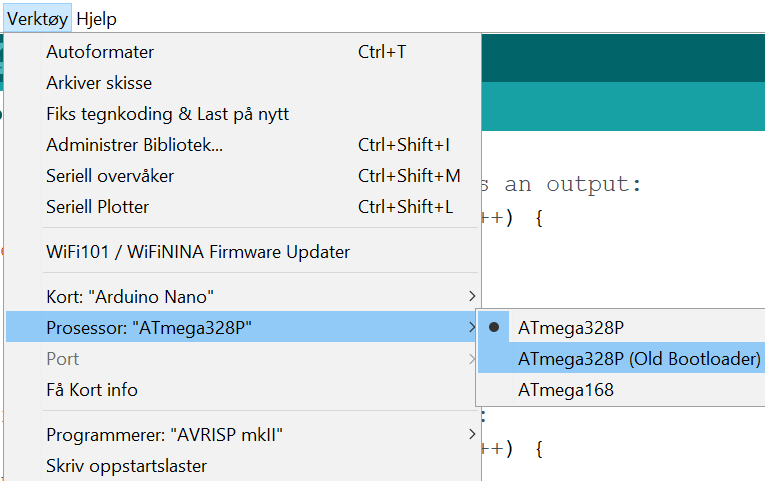
\includegraphics[width=10cm]{./lUltralydtransmitterx05.png}$$
\newpage
\begin{lstlisting}[language=Arduino]
// define the pins used for the HC-SR04.
const int trigger = 11;
const int echo = 10;

void setup
{
	// set pin functions
	pinMode(trigger,OUTPUT);
	pinMode(echo,INPUT);
}
void loop
{
	//first we trun off the trigger pin to be sure we have a clean high pulse
	digitalWrite(trigger, LOW);
	delayMicroseconds(2);
	//turn on the trigger pin for 10us
	digitalWrite(trigger, HIGH);
	delayMicroseconds(10);
	digitalWrite(trigger, LOW);
	// get time echo pin is on
	long duration = pulseIn(echo, HIGH);
	//recalculate time to distance
	float distance = duration * 0.0343 / 2;
}
\end{lstlisting}

Nå skal du ha et program som virker, men du har ingen måte å testet det på. Legg til funksjonalitet i programmet som gjør at du kan lese avstanden ut på seriemonitoren. Prøv også  å plotte den ut som en kurve. 

\subsection*{Oppgave 2 -  Oppkobling av 0.96" oled display}





\newpage

\underbar{file ./lUltralydtransmitter.tex}
\end{document}

